\documentclass[tikz,border=2pt]{standalone}
\usepackage{amsmath,amssymb}
\usepackage{tikz}
\usetikzlibrary{arrows.meta}

\begin{document}
% A network: vertices (cities, nodes) joined by edges (roads, links) carrying numbers such as
% lengths, costs or capacities.
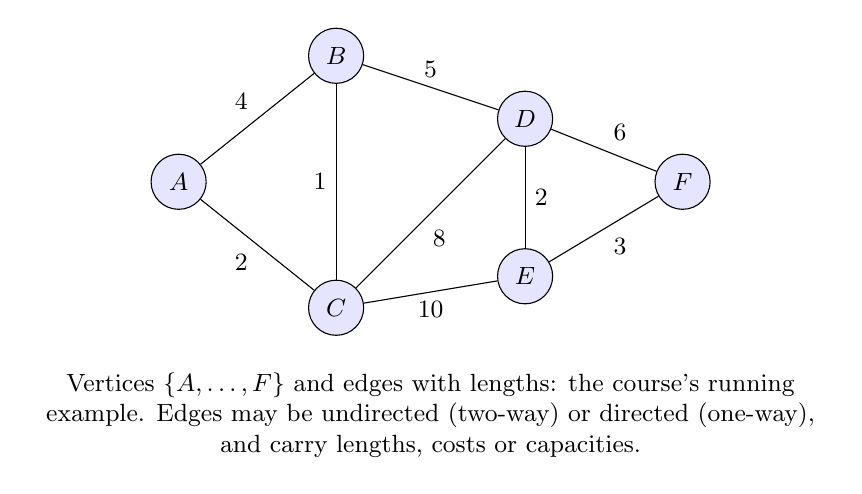
\begin{tikzpicture}[every node/.style={font=\small}, v/.style={draw, circle, fill=blue!10, minimum size=7mm, inner sep=0pt}]
	\node[v] (A) at (0,0) {$A$};
	\node[v] (B) at (2,1.6) {$B$};
	\node[v] (C) at (2,-1.6) {$C$};
	\node[v] (D) at (4.4,0.8) {$D$};
	\node[v] (E) at (4.4,-1.2) {$E$};
	\node[v] (F) at (6.4,0) {$F$};
	\draw (A) -- (B) node[midway, above left] {$4$};
	\draw (A) -- (C) node[midway, below left] {$2$};
	\draw (B) -- (C) node[midway, left] {$1$};
	\draw (B) -- (D) node[midway, above] {$5$};
	\draw (C) -- (D) node[pos=0.45, below right] {$8$};
	\draw (C) -- (E) node[midway, below] {$10$};
	\draw (D) -- (E) node[midway, right] {$2$};
	\draw (D) -- (F) node[midway, above right] {$6$};
	\draw (E) -- (F) node[midway, below right] {$3$};
	\node[anchor=north, align=flush center, text width=10cm] at (3.2,-2.3) {Vertices $\{A,\dots,F\}$ and edges with lengths: the course's running example. Edges may be undirected (two-way) or directed (one-way), and carry lengths, costs or capacities.};
\end{tikzpicture}
\end{document}
